\subsection{General Stuff}

For an energy-efficient PC, the cooling of the PC components plays a considerable role in the overall power consumption.
To get the most out of it, the cooling concept needs to be analyzed first. There are many arguments that speak for one or the 
other solution, which strongly depend on what is expected from the system.\\
Obviously, for example, a gaming/high-end PC needs more powerful cooling than an off-the-shelf office PC. While the high-end PC even needs
 a few case fans etc., a "cheap" case and no case fans will be enough for the office PC. \\
One of the more important requirements for a well-cooled PC, is the airflow. It transports the exhaust heat from the components (cpu, gpu etc.), away 
out of the case. If the airflow fails, the whole cooling fails, which can happen because of too much dust buildup or worn out fans. 
The components that need to be cooled usually, are the CPU and the GPU. Due to the porous nature of the surface of a cpu's/gpu's cooling plate, thermal
 grease needs to be applied, before mounting the heat sink.

\subsection{Thermal Grease}

As already mentioned before, thermal grease needs to be applied to increase the thermal conductivity between the surface of the cooling plate and the heat sink.
Without it, there would be uncountably many microscopic air-gaps between both surfaces. These gaps reduce the thermal conductivity considerably, since air is 
very bad heat conductor. Not to mention that those gaps would reduce the thermal conductivity in such a great deal, the heat couldn't be transported efficiently enough, resulting in 
overheating. \\
Following are the typical components in thermal grease, sorted by expensiveness in ascending order:

\begin{figure}[H]
  \centering
  \begin{tabular}{|l|l|}
    \hline
    type & thermal conductivity \\\hline\hline
    ceramic & 218 (beryllium oxide) \\\hline
    metal(silver, aluminium \dots) &  420 \\\hline
    carbon & \~900 \\\hline
    liquid metal (alloys) & ? \\\hline
  \end{tabular}
  \caption{types of thermal grease}
\end{figure}


As comparison, air has a thermal conductivity of 0.034. The thermal grease as whole has a conductivity between 0.5 and 10, depending on what product was used.
Resulting from the quality of the used grease, the temperature of the cooled component can vary by 2-5$^\circ$ C.

\begin{figure}[H]
  \centering
  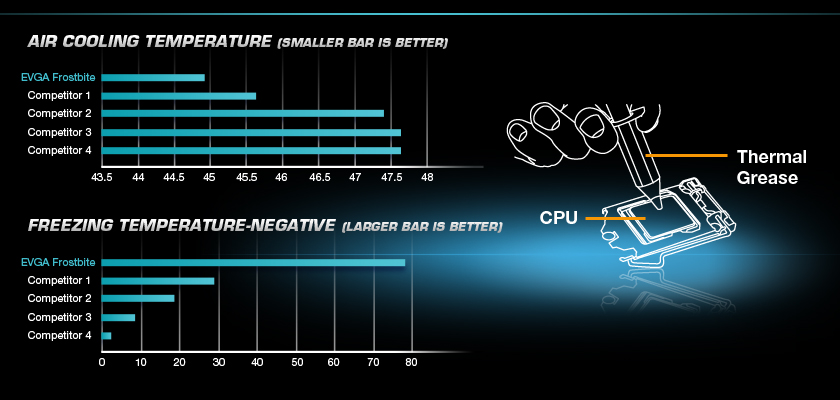
\includegraphics[width=1\textwidth]{./graphics/evga_frostbite_grease}
  \caption{comparison of thermal grease}
  \label{fig:grease_comparison}
\end{figure}


\subsection{Air Cooling}
Using conventional air cooling is the most common choice. It's accompanied by relative low effort, since the only thing needed is to mount the heatsink onto the cpu (after applying thermal grease).\\
Some advantages in using air cooling in PCs are:
\begin{compactitem}
\item fans are relatively cheap
\item easy to mount
\item no risk of damaging the components\\
\end{compactitem}
Disadavantages of air cooling are:
\begin{compactitem}
  \item fans can be loud
  \item mediocre cooling capabilities compared to other methods\\
\end{compactitem}

\subsubsection{Components to be cooled}
When using air cooling, at least the CPU needs a heatsink and depending on the TDP, an active fan, mounted onto the heatsink. Furthermore, modern GPU's need even bigger
heatsinks and fans than CPU's, although they are delivered with them mounted already, thus they need no further concern, except the airstream must reach the GPU to remove the heat.
The rest of the components may need cooling, although usually the airflow should help keep them cool enough. In high-end gaming PCs, a harddisk or even a memory cooler is neeeded.

\subsubsection{Types of cooler/fans}
A non-exhaustive list of typical cooler types are:
\begin{compactitem}
  \item cpu cooler
  \item gpu cooler
  \item case fan
\end{compactitem}
Depending on the quality of the heatsink, the CPU temperature can vary between 3 and 12$^\circ$C(see figure \ref{fig:comparison_fans} below). For an office PC, it usually suffices to use a relatively cheap CPU
with a low power consumption. If low enough, it may be possible to use a passive heatsink, which leads to saving a few watts and a more quiet computer.
The same can also be applied to energy-efficient graphics cards.
\\\\
Beside that, it's wise to mount at least 2 fans for cooling the components efficiently: one at the back or top of the case, sucking the hot air out of the case, and a second, 
sucking cold air in. This generates a constant stream of air, which transports the exhaust heat of the components out of the case.\\
Following diagrams should illustrate the differences in temperature between typical cpu coolers:\\
\begin{figure}[H]
  \centering
  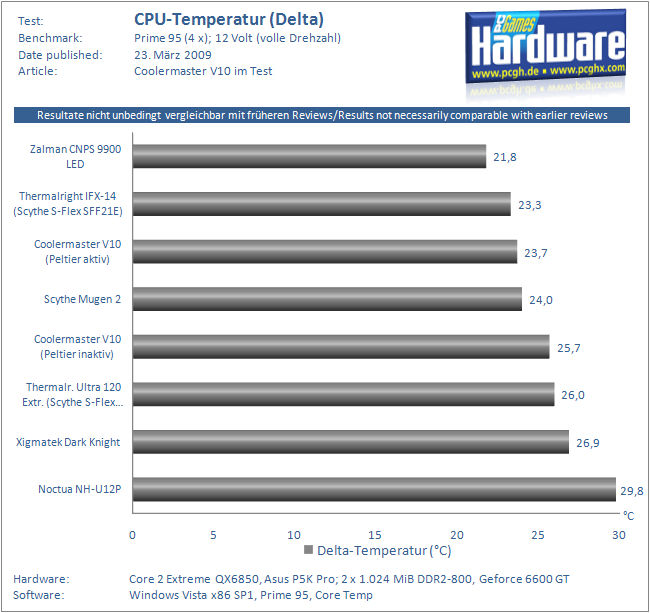
\includegraphics[width=0.7\textwidth]{./graphics/Temperatur}
  \caption{comparison of fans relative to the ambient temperature}
  \label{fig:comparison_fans}
\end{figure}
A fan has an energy footprint of about 2W - different fans by different manufacturers all have a similar power consumption, which is the reason, why there are no diagrams that compare them
in terms of power consumption. But in the end, the power consumption of the air cooling in a PC, is somewhere between 5(regular office PC) and 12W(gaming PC). Which is somewhat considerable, 
but doesn't make much difference to the overall power consumption. 

\subsection{Water Cooling}

Another method to cool PCs, which has some advantages compared to air cooling in terms of effectiveness is water cooling.
Since water has a thermal conductivity of 0.58 (remember, air has a thermal conductivity of 0.034), it's an about 10 times better thermal conductor than air.
Thus, water cooling does a much better job in transporting the exhaust heat away from the components, but this advantange is somewhat limited,
since the water still needs to be cooled with air. In the last few years, water cooling has been becoming more
common, since it's easer to install water cooling kits than it was in the past. \\
What's also remarkably, is the fact that several components can be cooled with the same system and the possibility of replacing the original GPU cooler
with a customized waterblock to reduce the loudness of the system. Here is a list of a few advantages and disadvantages\\
\begin{compactitem}
\item more silent
\item effective
\item less influence by the ambient temperature \\
\end{compactitem}
Disadvantages:
\begin{compactitem}
\item danger of coolant leak
\item components are more expensive
\item more work to install than conventional air cooling
\item more skill involved \\
\end{compactitem}

\subsubsection{Components involved in water cooling}

To build a water-cooled PC, at least the following components are required: radiator, waterpump, waterblock, watertank and tubes. 
One of the most important role in water cooling plays the water block, depending on the quality, the temperature may vary about 6 to 8$^\circ$C.
This is also reflected more or less by the price of a waterblock. They start at about \EUR{30} and can go up to \EUR{80} or \EUR{100} per block.\\
Obviously, the expensiveness of the components make water-cooling not always a viable choice for everyone. Water cooling usually makes only sense on heavily overclocked PCs, or for people who want their PC to be as silent as possible.\\
See figure \ref{fig:waterblocks_diff} below for a comparison of different waterblocks.

\begin{figure}[H]
  \centering
  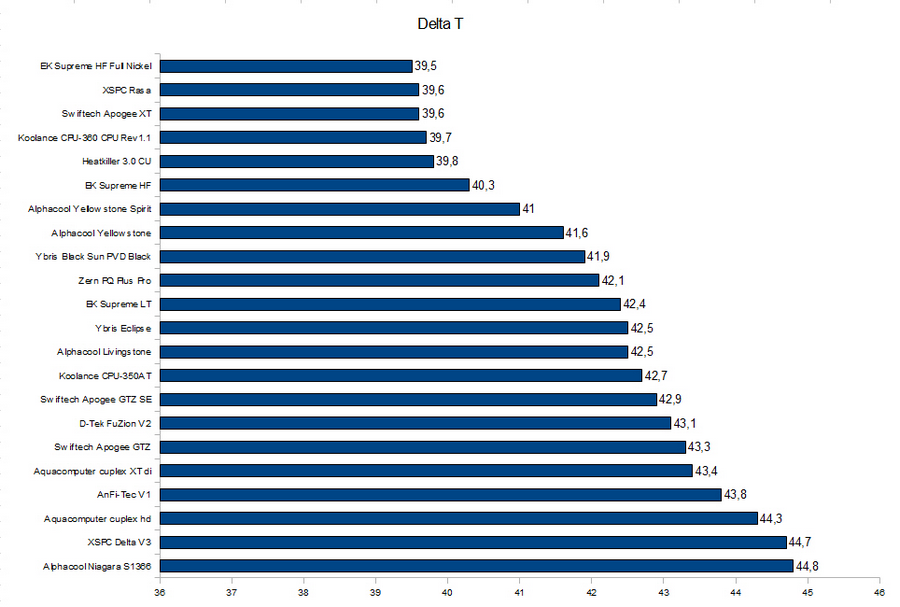
\includegraphics[width=.9\textwidth]{./graphics/waterblock_differences}
  \caption{temperature differences between waterblocks}
  \label{fig:waterblocks_diff}
\end{figure}
The next component, which will need the most power of a water-cooling system is the waterpump. Typical small waterpumps used for PCs will consume between 8 and 13W.
Including a 120mm fan, mounted on the radiator will consume (as mentioned above) between 2 and 4W. Depending on how much heat the PC generates, the radiator
needs more than 1 fan. Assuming 4 120mm fans are needed, the overall consumption of the cooling solution will amount to somewhere between 24 and 29W, which
is already relatively considerable. From this, it can be savely assumed that water-cooling only pays off, if conventional air-cooling measures don't suffice.

\subsubsection{water vs air}


Finally, a direct comparison of the temperatures between air and water cooling below:
\begin{figure}[H]
  \centering
  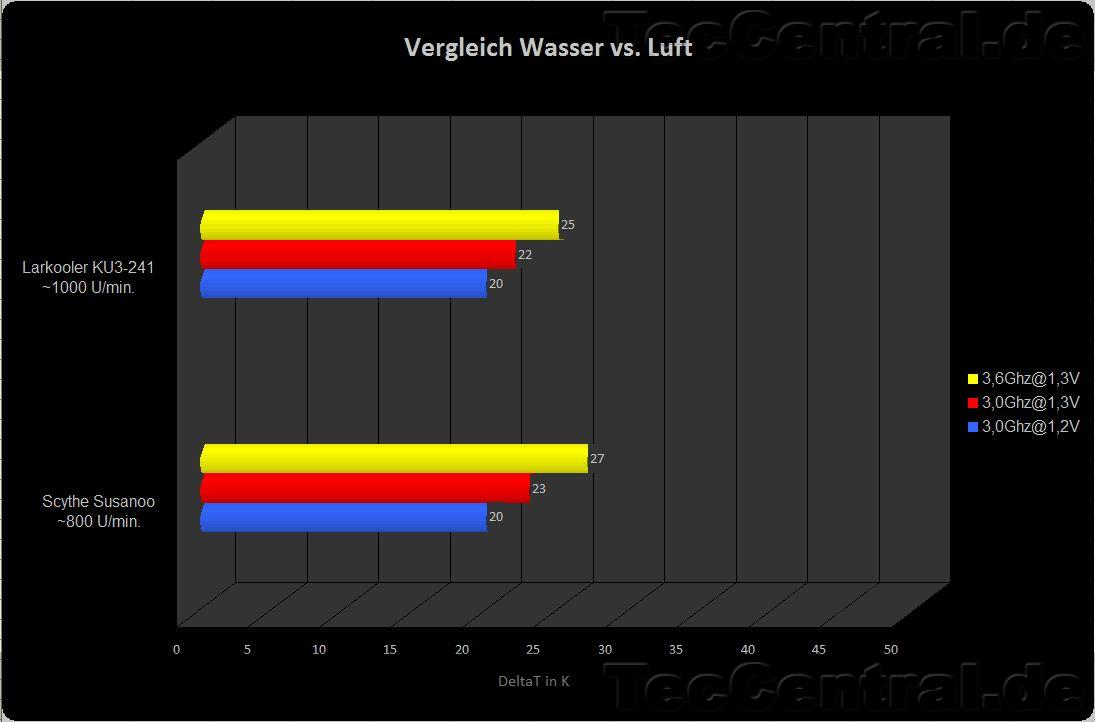
\includegraphics[width=.9\textwidth]{./graphics/water_vs_air.jpg}
  \caption{water vs. air\\}
  \label{fig:water_air}
\end{figure}
As can be seen in the diagram, water cooling makes only sense on overclocked systems. Only at 3.6 GHz, the water-cooled system is 2$^\circ$C lower than the air-cooled.
Considering the high costs for a water-cooled system and the higher maintenance, water-cooling is often not the optimal solution.


%%% Local Variables: 
%%% mode: latex
%%% TeX-master: "../template"
%%% End: 
